
\seciton{Topological knots}

Let $M$ be a manifold (we will assume $\dim M \ge 3$, since $2d$ and $1d$ is of
little interest), then an immersion $K \subset M$ of $S^1$, is called a
\wddef{topological knot}.  
\todo{Move this to a section on topological knots}
In the study of topological knots, one are interested in whether two knots are
equivalent. That is whether one knot can be turned into the another,
through a continues transformation. More precisely, 

\begin{defn}
Let $K$ and $K'$ be topological knots. An \wddef{isotopy} from $K$ to $K'$ is
map
\[ H : [0,1] \times S^1 \to M, \]
such $H(0,s^1) = K$, $h(1,S^1) = K'$ and for each $t\in [0,1]$, $H(t, S^1)$ is a
topological knot. (That is $H$ is a path from $K$ to $K'$ in the space of
topological knots in $M$. ) If such a map exists we say $K$ and $K$ are
\wddef{isotopic}.
\end{defn}

If $M = \R^3$, it is interesting to study the projections onto an embedded plane
$\R^2$. For almost all planes this projection will be \wddef{regular}, that is
injective except at a finite number of points.

\begin{lemma}
Considering the projection of an isotopy $H$ from $K$ to $K'$. Then $H$ consist
of continues deformations through regular knots as well as a finite number of so
called Reidemeister moves. There are three such Reidemeister moves, see figure
\pref{reid_moves_top}.
\end{lemma}


\begin{figure}
\centering
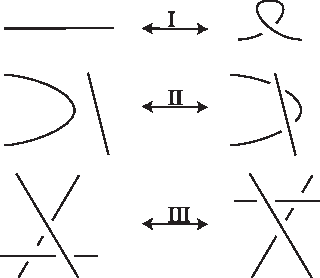
\includegraphics[width=.4\textwidth]{figs/reid_moves_top.pdf}
\caption{Topological Reidemeister moves}
\label{fig:reid_move_top}
\end{figure}
